\section{Rules Generation}
The first task we need to address is to generate the universe of all possible rules $R$ that covers one or more examples of the generation set $G$.
Recent KB rule mining approaches solve this aspect by loading the entire KB into main memory, and then discovering connections between entities by aggressively indexing KB triples on subject, object, and predicate~\cite{galarraga2015fast}(ANOTHER CITATION). These approaches work well with relatively small KBs. Unfortunately, modern KBs can easily exceed the size of hundread Gigas, which makes them too big to be entirely loaded into memory unless the whole process is run on a very powerful machine. We propose an alternative disk-based solution that loads into memory only portions of the KB that are needed for the target relation.

Given the generation set $G$, we can discover the universe of rules by just inspecting $G$. In fact, a rule that does not cover any element of $G$ will never be part of the optimal solution, since it does not give any contribution to the set cover problem.

\begin{figure}[t]
	\centering
	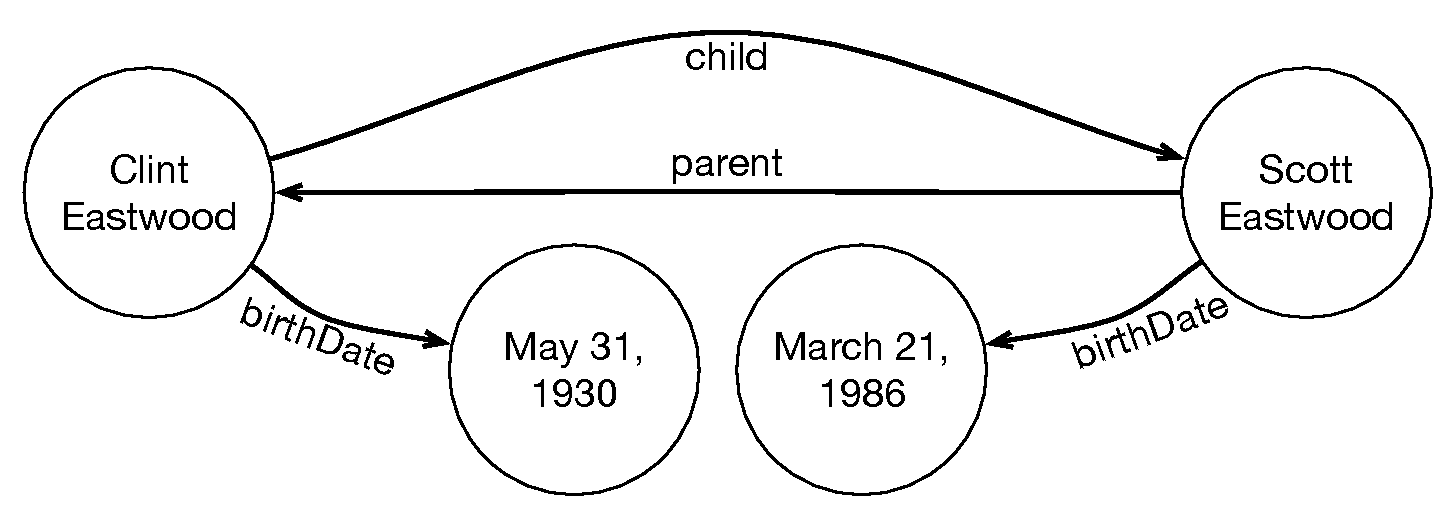
\includegraphics[width=\columnwidth]{include/figure/graph_example.pdf}
	\caption{Graph Portion of \dbpedia}
	\label{fig:graph_example}
\end{figure}

A KB $K$ can be straightforwardly translated into a directed graph: entities and literals are nodes of the graph, while there is a direct edge from node $a$ to node $b$ for each triple $\<a,rel,b\> \in K$. Edges are labelled, where the label is the relation $rel$ that connects subject to object. Figure~\ref{fig:graph_example} shows a portion of \dbpedia that connects two person in a child and parent relationship, along with their dates of birth. The graph represent information of four triples (two birth dates, one parent and one child).

The body of a Horn Rule can be seen as a path in the graph. W.r.t. Figure~\ref{fig:graph_example}, the body $\atom{child}{a}{b} \wedge \atom{parent}{b}{a}$ corresponds to the path \textit{Clint Eastwood} $\rightarrow$ \textit{Scott Eastwood} $\rightarrow$ \textit{Clint Eastwood}. In Section~\ref{sec:language} we defined valid rules. A valid body of a rule contains variables $a$ and $b$ at least once, and every other variable at least twice. 
In a valid body also each variable is connected transitevily to every other variable. 
If we allow the navigation of edges in any direction (no matter what the direction of the edge is on the graph), we can translate bodies of valid rules to paths on the graph.
Given a pair of entities $(x,y)$, a valid body corresponds to a path $p$ on the graph that meets the following criteria:
\begin{enumerate}
	\item $p$ starts at the node $x$;
	\item $p$ touches $y$ at least once;
	\item $p$ ends in $x$, in $y$, or in a different node that has been touched before.
\end{enumerate}
In other words, given the body of a rule $r_{body}$, $r_{body}$ covers a pair of entities $(x,y)$ iff there exists a path on the graph that corresponds to $r_{body}$. Therefore, given a pair of entities $(x,y)$, we can generate bodies of all possible valid rules by simpling computing all valid paths from $x$ with a simple BFS. Note how the transitevily connection between variables is always guaranteed by the construction properties of a path: for each node $n$ in the path there exists a subpath that connects $n$ to every other node in the path. The key is the ability of navigating each edge in any direction, which basically means turning the original directed graph into an undirected one.

Despite the navigation over an undirected graph, we still need to keep track of the original direction of the edges. This is essential when we want to translate a path to the body of a Horn Rule. In fact, if we have a direct edge $rel$ from $a$ to $b$, navigating the edge from $a$ to $b$ produces the atom $\atom{rel}{a}{b}$, while navigating the edge from $b$ to $a$ produces the atom $\atom{rel}{b}{a}$. These two atoms are different, where the position of variables is determined by the original direction of the edge.

One should notice that for two entities $x$ and $y$, there might exists infinite valid paths starting from $x$. Thus we introduce the $maxPathLen$ parameter that determines the maximum number of edges on the path. When translating paths to Horn Rules, $maxPathLen$ determines the maximum number of atoms that we can have in the body of the rule. This parameter is necessary to avoid the discovery of rules with infinite body lenght.

As we said above, our rules generation approach does not need to load the entire KB in memory. We can load in memory just the portion of the graph that is needed. Given a pair of entities $(x,y)$, we retrieve from the entire KB graph all the nodes at distance $maxPathLen-1$ or less from $x$ and $y$, along with the edges. Retrieving such nodes and edges can be done recursively: we mantain a queue of entities, and for each rntity in the queue we fire a SPARQL query to retrieve all entities at distance $1$ from the current entity (single hop queries). We add the new entities to the queue iff they are distance less than  $maxPathLen-1$ from either $x$ or $y$. The queue is initialised with $x$ and $y$. By doing so we load into memory only a small portion of the KB, the only one needed to discover rules that cover $(x,y)$. We will show in the experimental section that SPARQL engines are very fast at executing single hop queries.

The generation of the universe of all possible rules for a set $G$ is then straightforward: for each elemt $(x,y) \in G$, contruct the portion of the graph as described above and compute all valid paths starting from $x$. By computing paths for every example in $G$, we can also compute the coverage over $G$ for each rule. The coverage of a rule $r$ is the number of elements in $G$ where there exists a path that is equivalent to $r$. Path discovery will also generate single-instance rules: rules that cover only one example from $G$ by instantiating variables $a$ and $b$ in the rule. Once the universe of all possible rules has been generated (along with coverage over $G$), we can compute coverage and unbouned coverage over $V$ by simply executing two SPARQL queries against the KB for each rule in the universe. We will show in Section~\ref{sec:greedy_alg} how many queries can be avoided, as well as the generation of all possible rules.


\subsection{Literals and Constants}
We want a language to be powerful enough to include smarter comparison among literal values other than standard equalities, such as greater than or less than. In the path discovery approach, this translates on having edges that connect literal values with such kind of comparisons. As an example, Figure~\ref{fig:graph_example} should contain an edge '$<$' from node \textit{March 31, 1930} to node \textit{March 21, 1986}. Unfortunately the original KB does not contain this kind of information, and creating comparisons for all literals in the KB is unfeasible. Since we discover paths for a pair of entities in isolation, thus the size of a graph for a pair of entities is relatively small, we can afford to compare all literal values whithin the single example graph. This implies the creation a quadratic number of edges w.r.t. the number of literals in the graph. We will show in the experimental section that within a single example graph the number of literals is usually relatively small, thus the quadratic comparison affordable. Modern KBs include three types of literals: numbers, dates, and strings. Besides equality comparison, we add '$>$','$\geq$','$<$','$\leq$' relationships between numbers and dates, and $\neq$ among all literals. These new relationships are treated as atoms: $x \geq y$ is equivalent to $\atom{rel}{x}{y}$, where \texttt{rel} is equal to $\geq$.

We noticed that $\neq$ relation could be very useful for entities as well other than literals. Think about the following negative rule:
$$ \atom{bornIn}{a}{x} \wedge x \neq b \Rightarrow \neg \atom{president}{a}{b} $$
The rule states that if a person $a$ is born in a country that is different from $b$, then $a$ cannot be president of $b$. The rule holds for most of the countries in the world. To consider inequalities among entities, we could add artificial edges among all pairs of entities in the graph. This strategy however, despite being inefficient for the high number of edges to add, would lead to many meaningless rules. We notice that it is reasonable to compare two entities only when they are of the same type. All modern KBs include types information for every entity (often through the \texttt{rdf:type} statement), therefore we use this information. We add an artifical inequality edge in the graph only between those pairs of entities of the same type. In the above rule it makes sense to compare $x$ and $b$ because they are both countries.




\subsection{Input Examples Generation} \label{sec:examples_gen}
A crucial point for our approach is how to generate the two input sets $G$ and $V$, used to generate and validate rules. 

For an input KB $K$ and a relation $rel \in K$, we automatically generate a set of \emph{positive} examples ($P$) and a set of \emph{negative} examples ($N$). Positive examples are easy to generate: it is all the pairs of entities $(x,y)$ such that $\<x,rel,y\> \in K$ (all pairs of entities in a child relation if $rel$=child). Generating negative examples is slightly more complicated, since the closed world assumption does not longer hold in a KB. Differently from classic database scenarios, we cannot assume that everything that is not stated in a KB is false. Because of incompleteness, everything that is not stated in a KB is $unknown$ rather false. In order to generate negative examples we make use of a popular technique for KBs: \emph{Local-Closed World Assumption} (\emph{LCWA}) (REFERENCE). LCWA states that if a KB contains one or multiple object values for a certain subject and relation, then it contains all possible values (if a KB contains one or more child of Clint Eastwood, then it contains all the children). This is definitely for \emph{functional} relations (relations such as \emph{capital} where the subject can have at most one object value), it might not hold for non-functions (\emph{child}). Since KBs contain many non-functions relation, we extenf the definition of LCWA by considering the dual aspect: if a KB contains one or multiple subject values for a certain object and relation, then it contains all possible values. To generate negative examples we then take the union of the LCWA aspects: for a given relation $rel$, a negative example is a pair $(x,y)$ where either $x$ is the subject of one or more triples $\<x,rel,y'\>$ with $y \neq y'$, or y is the object of one or more triples $\<x',rel,y\>$ with $x \neq x'$. If $rel=child$, a negative example is a pair $(x,y)$ such that $x$ has some children in the KB that re not $y$, or $y$ is the child of someone that is not $x$. By taking the union we do not restrict relations to be functions (such as in~\cite{galarraga2015fast}). With this technique however, the number of negative examples could be very big (in the child relation is the cartesian product of all the people having either a child or a parent). We want to restrict the size and make it comparable to the size of positive examples. We therefore introduce another constraint, that significantly shrinks the size of negative examples: we require $x$ and $y$ to be in a relation in the original KB. This intution comes from how modern KBs are built: there is an automatic process that extracts data from some input sources according to pre-defined rules. If $x$ and $y$ are in a relation in the KB, then the KB construction should have been able to generate all possible relations between $x$ and $y$. If $x$ and $y$ are in one or more relations that is not the target relation, then most likely $x$ and $y$ are not in the target relation. This further restriction has multiple advantages: on the one hand it makes the size of negative examples of the same order of magnitude of positive examples (see Section~\ref{}), on the other hand it guarantees the existence of a path between $x$ and $y$, for every $(x,y)$ in the negative examples set. For positive examples, the existence of a path was already guaranteed since pairs in the positive examples set are connected by the target relation.

Once we generate positive and negative examples ($P$ and $N$), we can assign them to $G$ and $V$. When we discover positive rules (people that are in a child relation), we use $P$ as generation set $G$ and $N$ as validation set $V$. When we discover negative rules (people that are not in a child relation), we we use $N$ as generation set $G$ and $P$ as validation set $V$.

